\documentclass[12pt]{article}
\usepackage[utf8]{inputenc}
\usepackage{graphicx}
\usepackage{amsmath}
\usepackage{hyperref}
\usepackage{parskip}
\usepackage{xcolor}
\usepackage{sectsty}


% Define a custom blue color (modify RGB values to match your desired shade)
\definecolor{customblue}{RGB}{0, 51, 102} % Blue accent 1 dark 25% approximation


% Apply color to section titles
\sectionfont{\color{customblue}}

\begin{document}

{\color{customblue}\title{Predicting Customer Churn in E-Commerce}}
\author{Venkatesh Terikuti \\ Graduate}
\maketitle


\section*{Introduction}
In the competitive landscape of online retail, understanding customer behavior is pivotal for business success. A critical aspect of this understanding is identifying customer churn - a phenomenon where customers cease their relationship with the business. Predicting and analyzing churn can empower businesses to devise effective retention strategies. This project focuses on developing a churn prediction model using a dataset from a UK-based online retailer, aiming to identify customers at high risk of churning.

\subsection*{Machine Learning Algorithms}
To tackle this challenge, three robust machine learning algorithms were selected: Random Forest, known for accuracy and handling complex datasets; Support Vector Machine (SVM), ideal for high-dimensional feature spaces; and XGBoost, lauded for its speed and adaptability to diverse data. Each of these methods offers unique strengths in handling complex datasets and uncovering patterns, making them well-suited for predicting customer churn.

\subsection*{Dataset Overview}
The 'Online Retail II' dataset encapsulates transactional data from a UK-based online retailer, detailing transaction data from the online retailer, featuring attributes such as invoice number, stock code, description, quantity, invoice date, unit price, customer ID, and country. The primary challenges addressed include handling missing values, processing negative quantities, and transforming the data for predictive modeling of customer churn.

\section*{Explanation of Machine Learning Methods}
\subsection*{Random Forest}
\begin{itemize}
    \item Random Forest is an ensemble learning technique that builds multiple decision trees (D1, D2, ..., Dn) and merges them together to get a more accurate and stable prediction. Each tree in a random forest gives a prediction, and the final output is determined by majority voting in the case of classification or averaging in the case of regression.Individual decision trees are built on a randomly split subset of the training data. The split at each node of the tree is done on a random subset of features. The goal is to reduce overfitting of the model on the training set and improve generalization to unseen data. This is achieved by averaging or 'bagging' multiple trees to reduce variance without increasing bias significantly. The randomness in feature selection for splitting nodes helps in creating de-correlated trees, which, when averaged, reduce the model's variance. No single equation governs Random Forest; it's more about the algorithmic approach. Each tree is grown to the largest extent possible without pruning. For classification, the Gini impurity is often used to measure the quality of a split. Gini Impurity for a set is \( G = 1 - \sum (p_i)^2 \) where \( p_i \) is the probability of an item being classified into class i.
    \begin{center}
        \includegraphics[width=0.8\linewidth]{"C:/Users/ual-laptop/Downloads/Random Forest.png"} 
    \end{center}
\end{itemize}

\subsection*{Support Vector Machine (SVM)}
\begin{itemize}
    \item SVM is a supervised learning model that finds a hyperplane in an N-dimensional space (N = number of features) that distinctly classifies data points. The objective is to find a hyperplane with the maximum margin, i.e., the maximum distance between data points of both classes. In simple terms, SVM finds the line (in 2D) or plane (in higher dimensions) that separates classes with as wide a gap as possible.  The optimization problem in SVM is to maximize the margin between the closest points of the dataset, known as support vectors. This is formulated as a quadratic programming problem: Minimize \( \frac{1}{2} ||w||^2 \) subject to \( y_i (w \cdot x_i + b) \geq 1 \) for all i. \item For non-linearly separable data, kernel tricks are used to transform data into a higher dimension where a hyperplane can be used to separate the data. The decision function is \( f(x) = w \cdot x + b \). If \( f(x) \geq 1 \), the prediction is class 1; if \( f(x) \leq -1 \), it's class -1.
    \begin{center}
        \includegraphics[width=0.8\linewidth]{"C:/Users/ual-laptop/Downloads/SVM.png"}
    \end{center}
\end{itemize}

\subsection*{XGBoost}
\begin{itemize}
    \item XGBoost is a decision-tree-based ensemble Machine Learning algorithm that uses a gradient boosting framework. In prediction problems involving unstructured data (images, text, etc.), it is as good as deep learning. At each step, XGBoost adds a new tree that best reduces the loss (like Mean Squared Error for regression), using gradient descent. The model is built in a stage-wise fashion, and at each stage, it introduces a new tree to compensate for the deficiencies of existing trees. The objective function in XGBoost is given by: \( \text{Obj} = L + \Omega \) where \( L \) is the training loss function, and \( \Omega \) is the regularization term. \( L \) is typically a log loss for classification and Mean Squared Error (MSE) for regression. \( \Omega \) consists of the number of leaves in the tree and the square of the magnitude of leaf weights, introducing a penalty for complexity.
    \begin{center}
        \includegraphics[width=0.8\linewidth]{"C:/Users/ual-laptop/Downloads/XGBoost.png"}
    \end{center}
\end{itemize}

\section*{Data Preprocessing and Model Development}

\subsection*{Data Preprocessing}
The "Online Retail II" dataset served as the groundwork for our study, containing rich transactional information characterized by features such as invoice number, stock code, description, and others. A thorough preprocessing routine was indispensable to ensure data integrity and utility.

\medskip % Adds a medium space
One of the initial steps was the meticulous management of missing values, a prevalent quandary in data analytics. Specifically, we purged records lacking 'Customer ID', which is indispensable for individual customer analysis. For the 'Description' attribute, we imputed missing values with the mode, thus preserving the dataset's integrity for product-centric evaluations.

\medskip
We also discarded transactions with negative quantities, which typically denote returns or cancellations, to focus exclusively on actual purchase data. This was a deliberate choice to ensure the accuracy of subsequent behavioral analyses, particularly regarding customer churn.

\medskip
Feature engineering was a focal point of this stage, leading to the formulation of the 'TotalPrice' feature—calculated by multiplying 'Quantity' and 'Price'. This enriched the dataset by encapsulating each customer's expenditure profile at a granular level, encompassing their total spend, average transaction value, and frequency of purchases. The derived attribute 'Days Since Last Purchase' provided a measure of customer engagement, acting as a potential churn predictor.

\medskip
We allocated 70\% of the dataset for model training and reserved the remaining 30\% for testing, following conventional data splitting practices. Such a distribution balances the need for model training comprehensiveness with adequate evaluation capacity.

\subsection*{Model Development}
The feature set underwent standardization using the StandardScaler to normalize the data, a necessary precondition for SVM's optimal performance due to its sensitivity to the scale of input features.

\medskip
Our choice of machine learning models for the classification task was motivated by their respective track records in predictive accuracy and efficiency. The Random Forest Classifier was a prime candidate, renowned for its effectiveness with complex and imbalanced datasets. The SVM with a linear kernel was expected to perform admirably in high-dimensional spaces, which are typical of retail transaction datasets. Lastly, the inclusion of the XGBoost Classifier was driven by its speed and state-of-the-art performance, which are indispensable for managing datasets with a vast feature space.

\medskip
The training phase involved each model being fed with the standardized training data. Default hyperparameter settings were used initially, laying the groundwork for subsequent fine-tuning. Hyperparameter optimization is often critical to model performance, and it was here where cross-validation played a pivotal role.

\section*{Cross-Validation and Model Optimization}
Employing a 5-fold cross-validation approach provided a stringent and multifaceted evaluation of each model. This not only appraised the models' efficacy but also their adaptability to unseen data—a safeguard against overfitting. Moreover, cross-validation assured a thorough vetting of the models' real-world applicability, a testament to their anticipated operational reliability.

\medskip
The culmination of this phase was a comprehensive set of models, each offering unique insights and predictive capabilities. The subsequent sections of the report will delve into the outcomes of the evaluation phase, contrasting model performances, and interpreting feature importance results. These insights will inform the final selection of the model or models that best meet the project's objectives and the practical considerations of deployment in a live retail environment.

\section*{Evaluation}
The evaluation of the machine learning models was meticulously structured to ensure a comprehensive understanding of their performance and applicability to the problem of customer churn prediction. This stage was crucial in determining the efficacy of the models in real-world scenarios.

\subsection*{Evaluation Methodology}
Our evaluation methodology encompasses the assessment of model performance and the understanding of feature relevance. We adopted accuracy, sensitivity, and specificity as our primary performance metrics. These metrics were selected to capture both the general correctness of the model and its ability to correctly identify positive and negative instances.

\subsection*{Performance Metrics}
Accuracy provides a straightforward measure of overall model performance. Sensitivity, also known as recall, gauges the model's ability to identify positive cases, which is crucial when the cost of false negatives is high. Specificity measures the identification of negative cases, equally important when false positives carry significant consequences. These metrics offer a balanced view of model performance, especially in scenarios where the datasets might be imbalanced or when different types of classification errors have different implications.

\subsection*{Cross-Validation}
To ensure that our models' performance metrics are not a result of overfitting, we employed 5-fold cross-validation. This technique partitions the dataset into five subsets, using four for training and one for validation, rotating until each subset has served as the validation set. The mean performance across folds provides a more reliable estimate of the model's performance on unseen data. This method not only strengthens the validity of our performance estimates but also ensures the models' stability across various subsets of data.

\subsection*{Feature Importance Analysis}
Feature importance provides insights into which features most strongly influence the model's predictions. For Random Forest, we relied on the intrinsic feature\_importances\_ attribute. For the linear SVM, we used the model coefficients (coef\_ attribute), and for the non-linear SVM (RBF kernel), we implemented permutation importance. This analysis helps us understand which features the models are focusing on and which features might be less informative.

\bigskip % Adds a bigger space before the graphs
% Graph 1
\begin{figure}[!htbp]
\centering
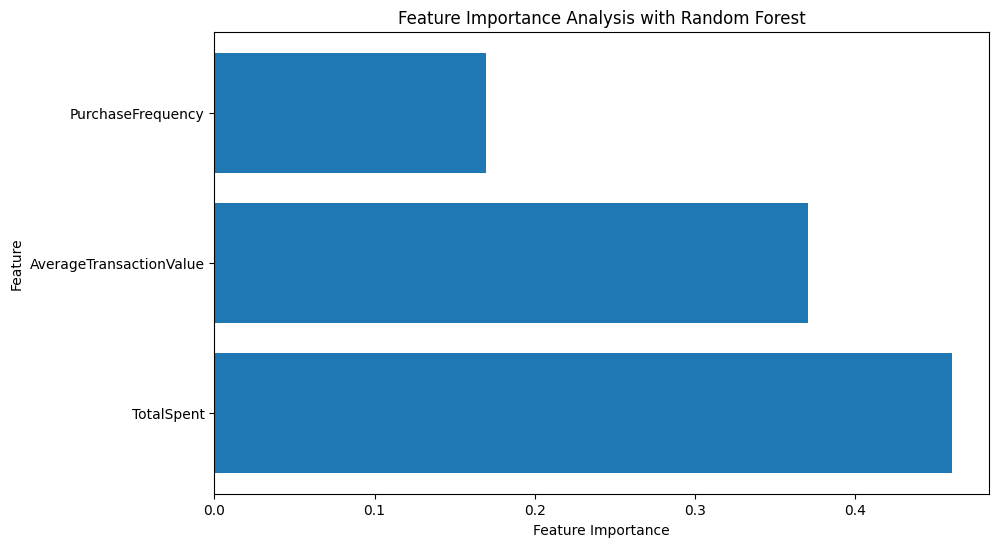
\includegraphics[width=0.8\linewidth]{"C:/Users/ual-laptop/Downloads/rf.png"}
\caption{Feature Importance Analysis with Random Forest}
\label{fig:graph1}
\end{figure}

% Graph 2
\begin{figure}[!htbp]
\centering
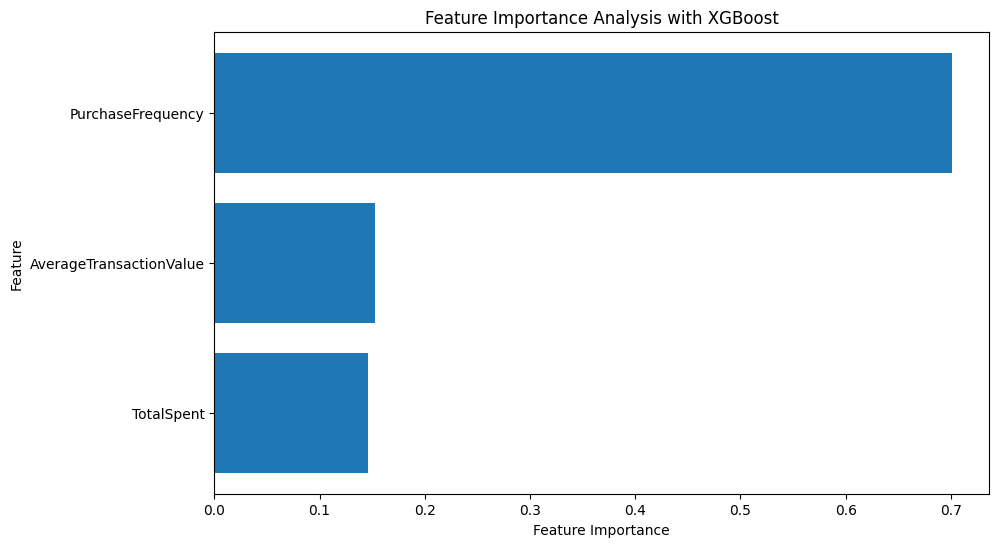
\includegraphics[width=0.8\linewidth]{"C:/Users/ual-laptop/Downloads/xgb.png"}
\caption{Feature Importance Analysis with XGBoost}
\label{fig:graph2}
\end{figure}

% Graph 3
\begin{figure}[!htbp]
\centering
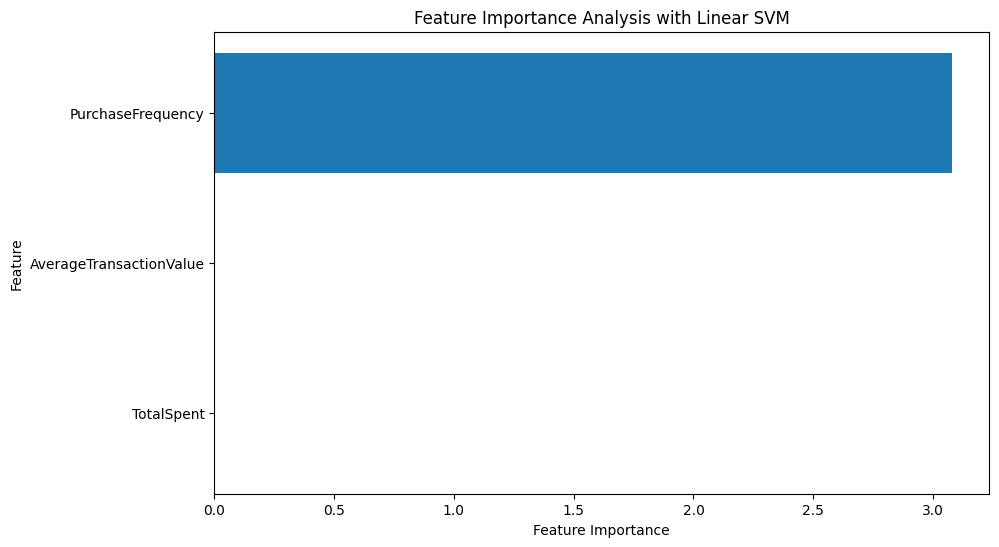
\includegraphics[width=0.8\linewidth]{"C:/Users/ual-laptop/Downloads/svm1.png"}
\caption{Feature Importance Analysis with Linear SVM}
\label{fig:graph3}
\end{figure}

% Graph 4
\begin{figure}[!htbp]
\centering
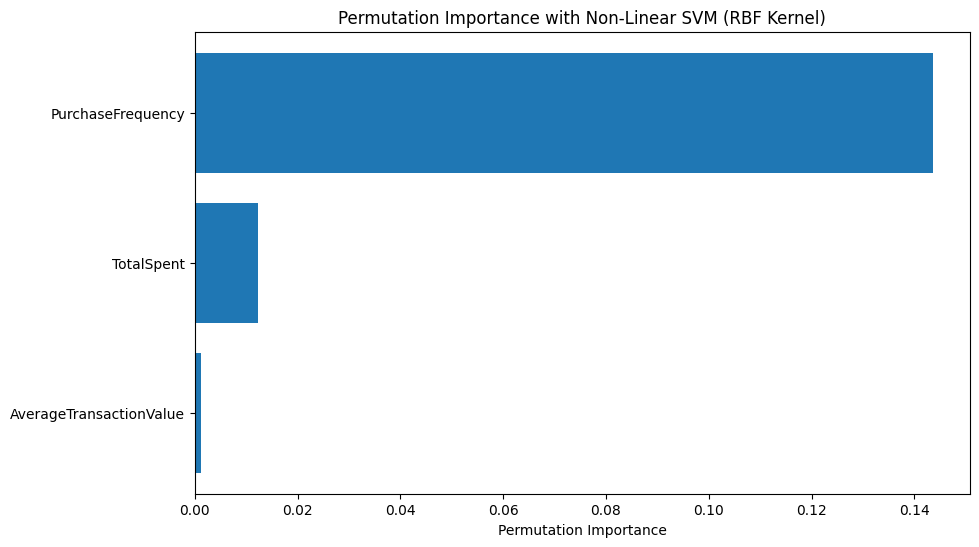
\includegraphics[width=0.8\linewidth]{"C:/Users/ual-laptop/Downloads/svm2.png"}
\caption{Feature Importance Analysis with Gaussian(Non Linear) SVM}
\label{fig:graph4}
\end{figure}

\clearpage

\section*{Evaluation Results}
The output from the execution of our models provided the following insights:

\medskip
\begin{itemize}
    \item XGBoost demonstrated accuracy scores ranging from 66.06\% to 68.84\% with sensitivity from 69.97\% to 74.60\%. The specificity varied slightly from 62.12\% to 63.03\%, with cross-validation scores averaging at 67.61\% initially, improving to 70.41\% after hyperparameter tuning.
    \item Random Forest showed a consistent accuracy improvement from 65.38\% to 69.35\%, with sensitivity increasing from 67.16\% to 75.85\% and specificity marginally improving. Cross-validation scores averaged at 67.10\% initially, rising to 70.36\% after tuning, indicating a stable performance across folds.
    \item SVM (Linear Kernel) achieved the highest accuracy of 68.44\%, with a notable sensitivity of 86.91\% but a lower specificity of around 49.83\%. The cross-validation average was 68.22\%, showcasing its robustness across different data splits.
    \item SVM (RBF Kernel) produced accuracy and sensitivity close to the linear kernel but with slightly improved specificity. The average cross-validation score for the Gaussian SVM was the highest at 69.99\%, suggesting a strong and consistent performance.
\end{itemize}

\medskip
\section*{Comparative Analysis}
When comparing the models, SVM (linear kernel) showed high sensitivity, indicating a strong ability to predict true positives but at the cost of many false positives, as reflected in the lower specificity. The non-linear SVM (RBF kernel) balanced this with improved specificity while maintaining high sensitivity.

\medskip
Random Forest and XGBoost presented more balanced performances across all metrics, with XGBoost slightly outperforming Random Forest in sensitivity and Random Forest catching up post-tuning. In terms of feature importance, all models agreed on the significance of PurchaseFrequency. However, Random Forest placed more emphasis on TotalSpent, differing from the linear models, which could be attributed to the ensemble method's ability to capture complex interactions between features.

\medskip
\section*{Conclusion}
The evaluation of the three machine learning models on our dataset reveals that each model offers unique strengths. XGBoost and Random Forest are more balanced in terms of sensitivity and specificity, while SVM, particularly with the linear kernel, excels in sensitivity, suggesting different use-case applicability. Feature importance analysis underscores PurchaseFrequency as a key predictor across models, with other features displaying varying degrees of influence. The choice of model for deployment would thus depend on the specific performance requirements of the application and the relative costs of false positives and negatives.

\medskip
\section*{Citations and Background Material}
\begin{itemize}
    \item Breiman, L. (2001). "Random Forests." Machine Learning, 45(1), 5-32. This paper is foundational for understanding the development and functioning of the Random Forest algorithm.\\
    url: \url{https://link.springer.com/article/10.1023/A:1010933404324}

    \item Cortes, C., \& Vapnik, V. (1995). "Support-Vector Networks." Machine Learning, 20(3), 273-297. This work by the creators of SVM provides an in-depth theoretical foundation for the algorithm.\\
    url: \url{https://link.springer.com/article/10.1007/BF00994018}

    \item Burges, C. J. C. (1998). "A Tutorial on Support Vector Machines for Pattern Recognition." Data Mining and Knowledge Discovery, 2(2), 121-167. This tutorial offers a comprehensive introduction to SVMs, particularly in the context of pattern recognition.\\
    url: \url{https://www.microsoft.com/en-us/research/wp-content/uploads/2016/02/svmtutorial.pdf}

    \item Chen, T., \& Guestrin, C. (2016). "XGBoost: A Scalable Tree Boosting System." In Proceedings of the 22nd ACM SIGKDD International Conference on Knowledge Discovery and Data Mining (pp. 785-794). This paper details the technical aspects and advancements of XGBoost.\\
    url: \url{https://dl.acm.org/doi/pdf/10.1145/2939672.2939785}

    \item Rogers, S., \& Girolami, M. (2016). "A First Course in Machine Learning." Although XGBoost might not be covered extensively in this textbook, the book lays down fundamental concepts of gradient boosting and decision trees that are central to understanding XGBoost.\\
     \item Dataset source: \url{https://archive.ics.uci.edu/dataset/502/online+retail+ii}
\end{itemize}


% ... [End of document] ...

% Continue with other sections as needed

\end{document}
